\documentclass[a4paper, amsfonts, amssymb, amsmath, reprint, showkeys, nofootinbib, 12pt]{article} %twoside
\usepackage[english]{babel}
\usepackage[utf8]{inputenc}
\usepackage{amsmath}
\usepackage[colorinlistoftodos, color=green!40, prependcaption]{todonotes}
\usepackage{minted} \usepackage{tcolorbox} \tcbuselibrary{minted}
%\usepackage{enumitem} \setlist{noitemsep}
\usepackage{listings}
% setup figure captions
\usepackage[font={small,it}]{caption}
% allow hard figure placement
\usepackage{float}

\usepackage[pdftex, pdftitle={Article}, pdfauthor={Author}]{hyperref} % For hyperlinks in the PDF
%% Sets page size and margins
\usepackage[a4paper,top=2cm,bottom=2cm,left=2cm,right=2cm,marginparwidth=2cm]{geometry}

% \begin{code}{python} ... \end{code}: environment for displaying code
\newtcblisting{code}[2][]{ %linenos can be put in options
  minted options={mathescape,fontsize=\footnotesize,numbersep=5pt},  
  minted language=#2,
  #1,
  listing only
}

% make hyperlinks be blue
\usepackage{hyperref}
\hypersetup{
    colorlinks=true,
    linkcolor=blue,
    filecolor=blue,      
    urlcolor=blue,
}
\urlstyle{same}

% set indentation size for whole document
\setlength\parindent{24pt}
% use RaggedRight for raggedright with indentation
\usepackage{ragged2e}
\setlength{\RaggedRightParindent}{\parindent}

% signature line
% \usepackage{showframe}
% \newcommand*{\SignatureAndDate}[1]{%
%     \par\noindent\makebox[2.5in]{\hrulefill} \hfill\makebox[2.0in]{\hrulefill}%
%     \par\noindent\makebox[2.5in][l]{#1}      \hfill\makebox[2.0in][l]{Date}%
% }%

% make references appear in table of contents
%\usepackage[nottoc,numbib]{tocbibind}

% change figure caption to FIG instead of figure
\makeatletter
\renewcommand{\fnum@figure}{FIG. \thefigure}
\makeatother

\begin{document}
\title{Sooner Competitive Robotics}
\author{The University of Oklahoma \\ ``The Aluminum Whale''}
\date{Submitted May 22nd, 2021}

\maketitle
%\tableofcontents

\centering
%{\color{red} DOPE CAD MODEL OF ROBOT}
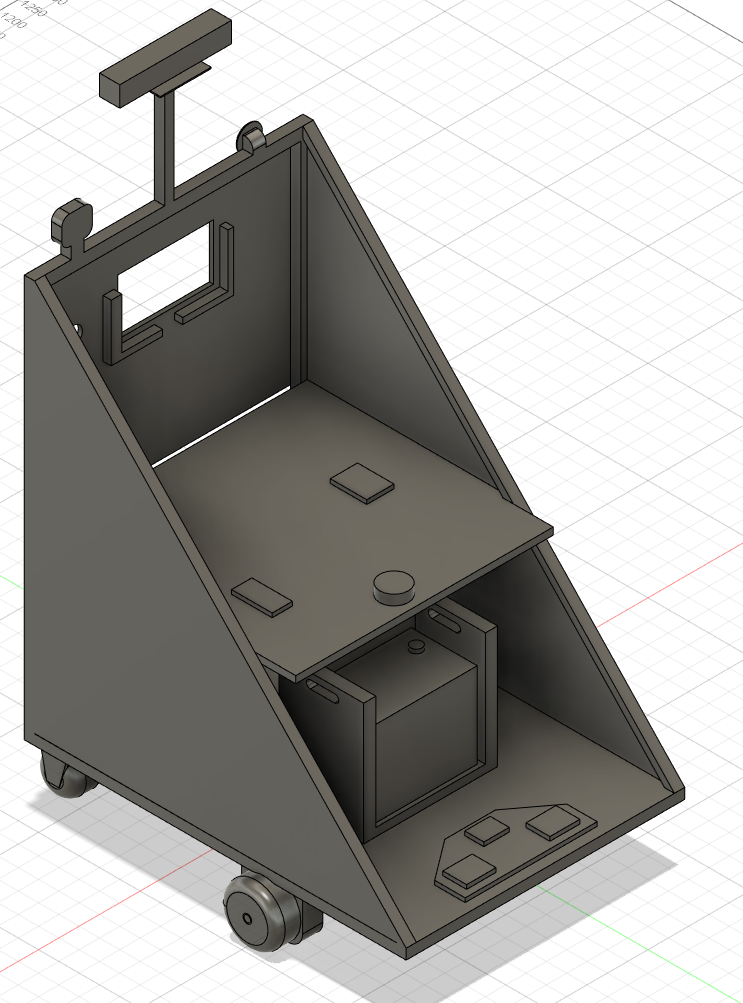
\includegraphics[width=0.4\textwidth]{images/frame/frame4.PNG}

\begin{center}
Team Captain: Kevin Robb \\
The Team: \\
\vspace{.2in}
\begin{tabular}{|c c c|}
    \hline
    Kevin Robb & kevin.robb@ou.edu & Undergrad \\
    Noah Zemlin & noah.zemlin@ou.edu & Grad \\
    Tyler Julian & tyler.james.julian@ou.edu & Grad \\
    Jorge Exinia & exinia@ou.edu & Undergrad \\
    Kichang Song & ksong@ou.edu & Undergrad \\
    Sarah Brown & srb@ou.edu & Undergrad \\
    Stephanie Sheldon & scs@ou.edu & Undergrad \\
    \hline
    Dr. Chad Davis & weeb@ou.edu & Advisor \\
    \hline
\end{tabular}
\end{center}

{ % use special formatting just for the certification statement
\hyphenpenalty=10000
\exhyphenpenalty=10000
\noindent
I certify that the design, development, and work put towards this project by the Sooner Competitive Robotics students is significant and equivalent to a senior design course.
}

% paragraph formatting style for whole document
\RaggedRight

% signature line for chaddy daddy
\vspace{.2in}
{\Large X}
\vspace{.05in}
\hrule


\clearpage
\section{Team Introduction}

We are Sooner Competitive Robotics (SCR) at the University of Oklahoma. Our organization has existed since 2013, and we have competed all over the U.S. since then. We intended to participate in the IGVC AutoNav challenge in 2020, but since it was canceled, this will be our first time competing. 

Our robot is called the Aluminium Whale. Last year, our chassis was a heavy steel frame that we struggled to push and carry around, so we called it the Steel Cannon. This year, we used aluminum for our main frame, with most paneling being acrylic, so the robot is much lighter. When doing our first outdoor drive test, we found that our clearance between the underside of the base and the ground was so small that the robot could easily become ``beached'' on the edges of sidewalks or even small perturbations in the height of the dirt. This led us to a name within the same naming scheme as its predecessor, the Aluminum Whale. (We've improved our clearance since then, so we hope this namesake will not be demonstrated during the competition). 

\begin{figure}[h]
    \centering
    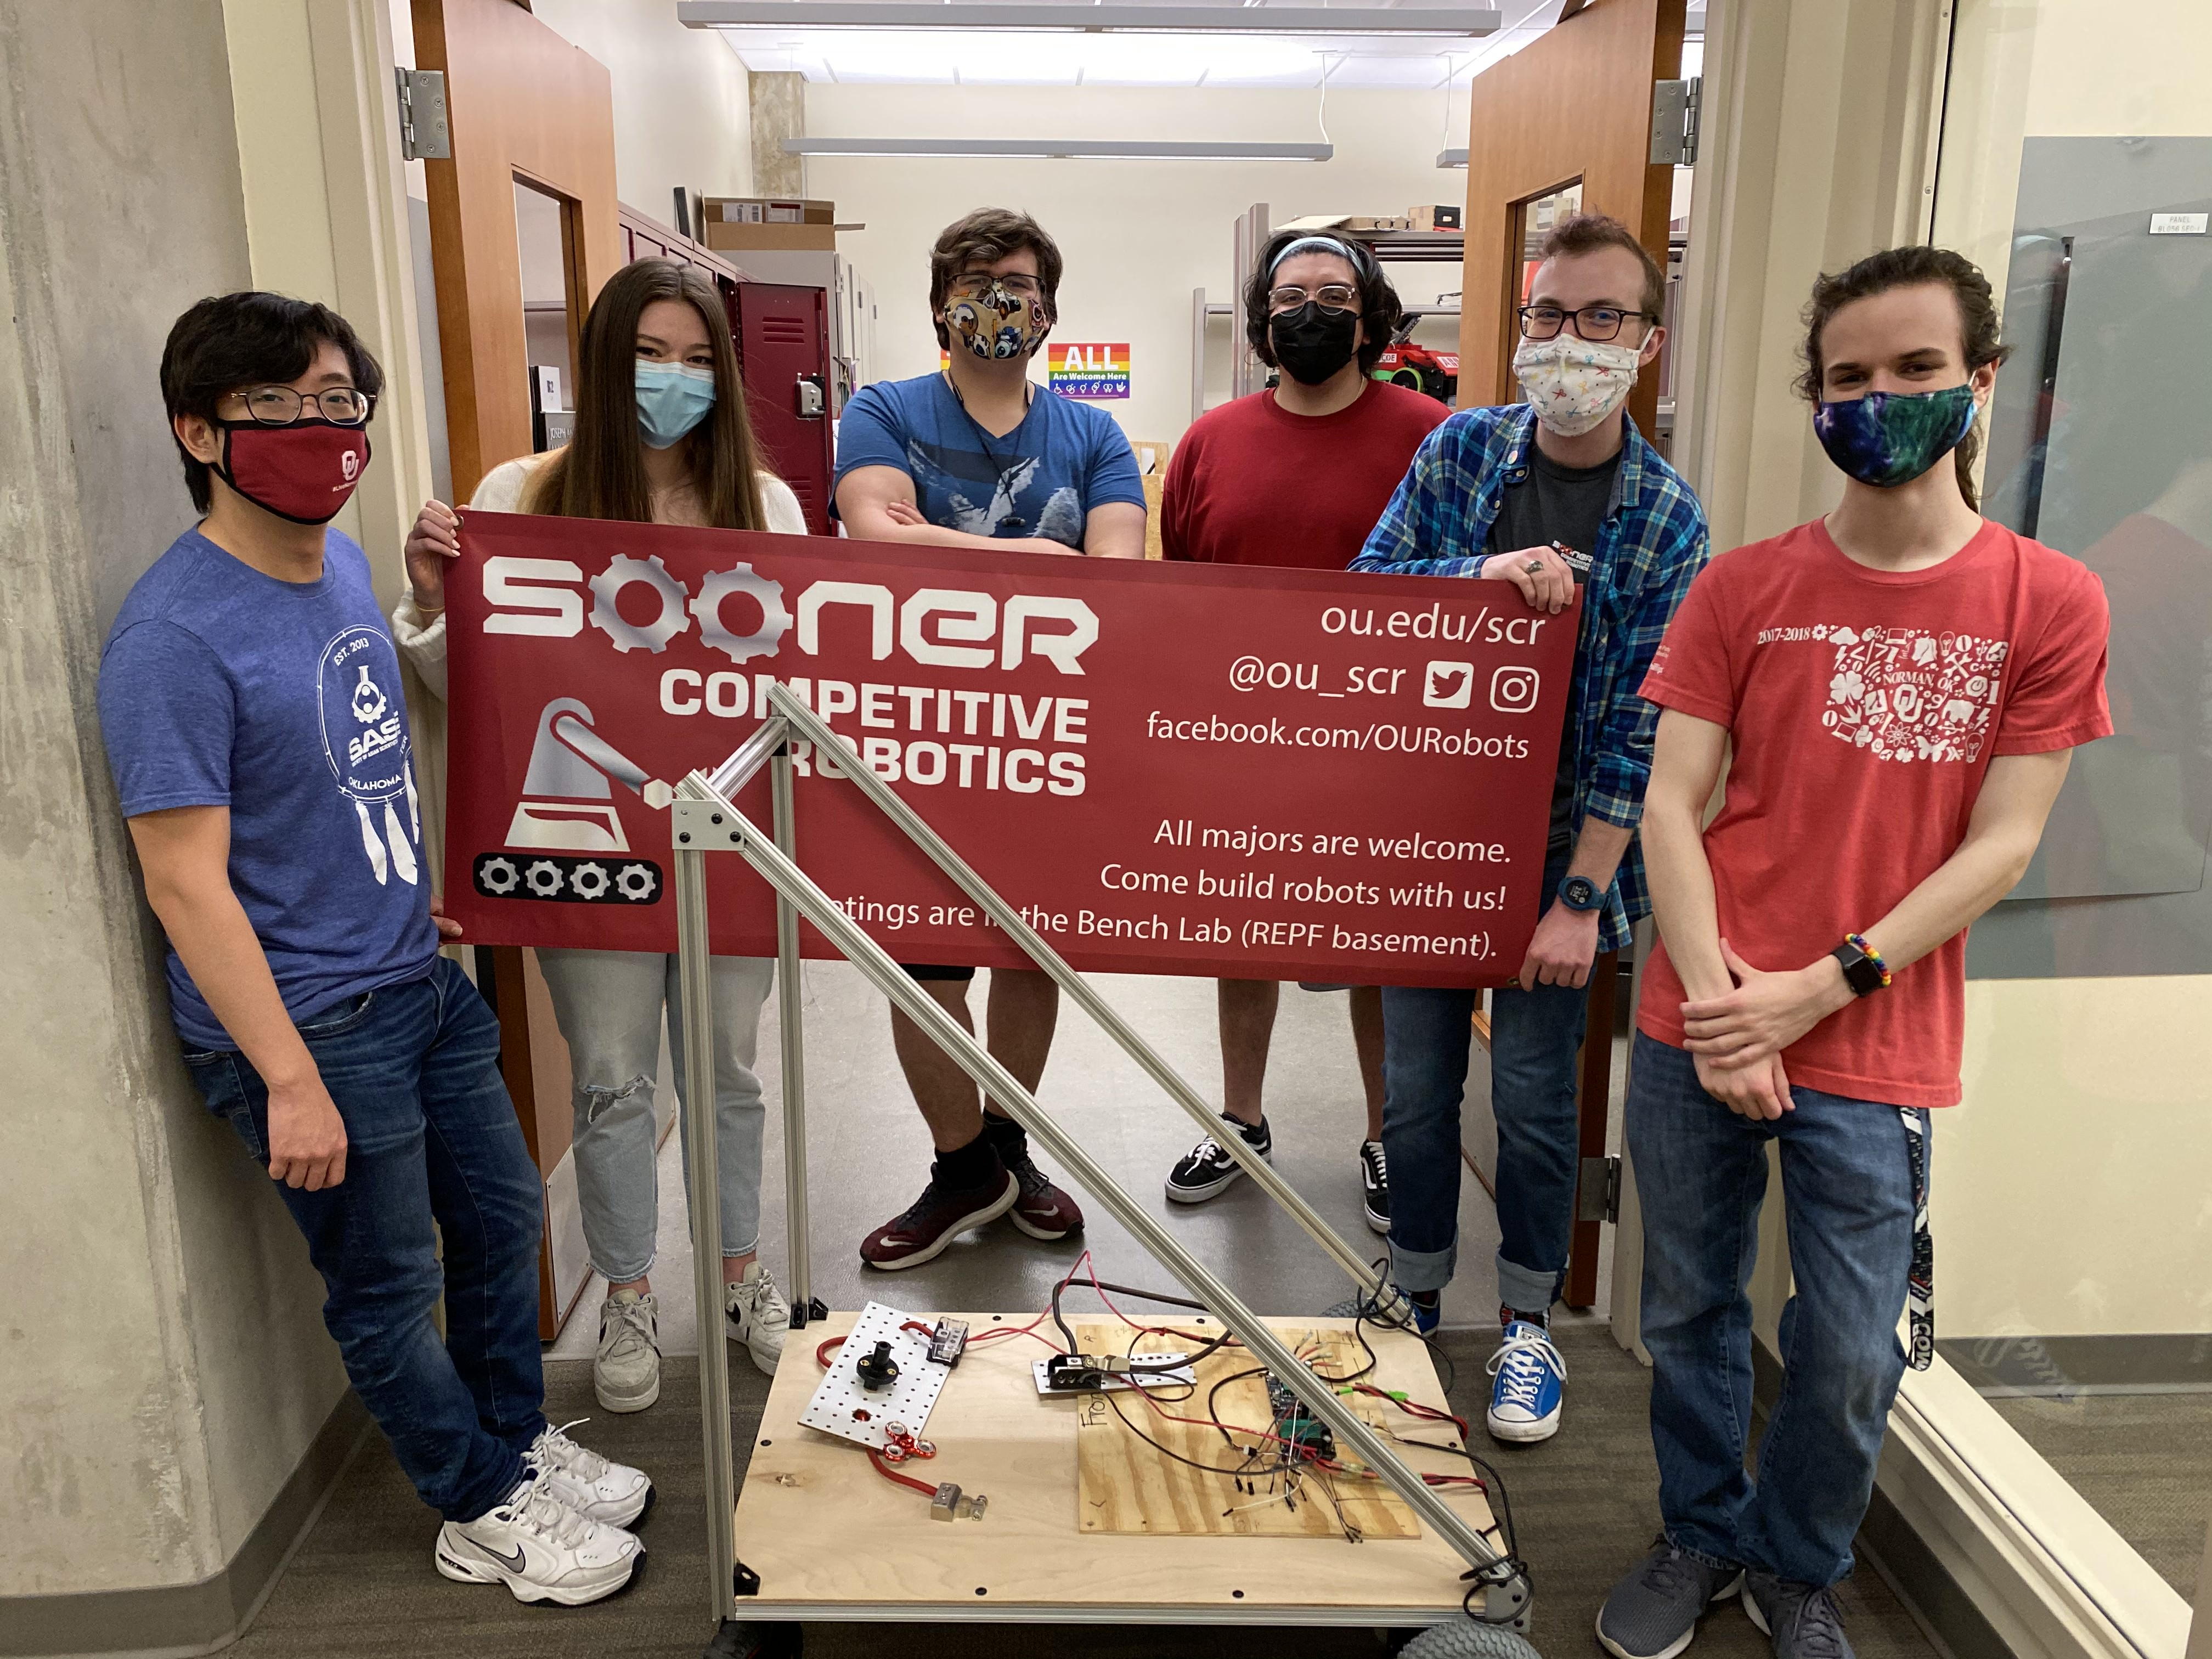
\includegraphics[width=0.5\textwidth]{images/team.jpg}
    \caption{The team with an early version of the robot.}
\end{figure}

The team was organized into three subteams (software, electrical, and mechanical), but membership on these teams was not mutually exclusive. Since our team is so small, many of our members contributed to multiple areas throughout our build process. The following table shows each member with their area(s) of contribution (S=Software, E=Electrical, M=Mechanical). 

\begin{center}
\begin{tabular}{|c c|}
    \hline
    Kevin Robb & S/M \\
    Noah Zemlin & S/E/M \\
    Tyler Julian & E/M \\
    Jorge Exinia & E/M \\
    Kichang Song & S \\
    Sarah Brown & E \\
    Stephanie Sheldon & M \\
    \hline
\end{tabular}
\end{center}

We identify Software contributions as significant work towards the code for part of the robot’s autonomous operation or other functionality.  Firmware creation is classified under Electrical. Work with PCB design, wire routing, and everything else in that realm falls under Electrical. Mechanical work includes design and construction of the main robot, 3D modeling, and printing of mounts and other parts, and considerations such as robot leveling, squaring, and weight distribution.


\clearpage
\section{Design and Strategy Overview}

\subsection{Assumptions and Priorities}

Our goal was to create a robot that can reactively avoid obstacles, stay in the lanes, and make reasonable progress through the course. We held off on our more ambitious software goals that would mainly help us in No Man's Land until we were confident that we'd be able to make it there in the first place. Similarly, we didn't worry about the ramp until we were confident we'd be able to make it to the ramp.

We wanted our camera to have an easy view of the relevant part of the course and also have the robot's front wheels in the frame to help with recognizing if we're in the lanes or not. This goal led our design process for the physical robot to the wedge shape we have now, with the camera up high at the rear, looking down the slant.

In our internally generated local map of the course, the robot is represented by only a single point, and to compensate for this, all obstacles are expanded radially by the maximum radius of the robot. This massively simplifies our navigation while still preventing collisions and using a relatively simple algorithm for local path planning. To make this viable, our robot needs to turn as close to in-place as possible, so our main drive wheels are near the center point of the robot.

We also knew that our entire robot would need to be able to hard shut down at the press of the onboard or remote E-stop buttons. We figured the remote is a convenient way to control the robot during testing, so we decided to include a mobility stop as well. The difference here is the E-stop requires the robot to be restarted entirely to operate again, while the mobility stop is reversible for our testing.

\subsection{Innovations} \label{sec:innovations}
The prime innovations for our electrical team were integrating the CAN bus communication protocol and using custom PCBs with STM32 microcontrollers. The CAN bus is a reliable and safe two-wire communication protocol that is heavily used in the automotive industry. The significant upside to the CAN bus is that no host computer controls everything, so the robot is still functional when a module malfunctions. The only major downside of using the CAN bus is that most development boards do not have CAN transceivers integrated; we chose to create custom PCBs for our modules with built-in CAN transceivers and STM32 microcontrollers, so this was not an issue for us.

The innovative aspects of our software team were the use of a convolutional neural network (CNN), a type of machine learning, to autonomously learn the best algorithm for lane detection. This can outperform anything we could have implemented manually, such as thresholding. Another innovative aspect was the creation of an entirely custom simulator to use for testing the software for this robot, which is detailed much further in Section \ref{sec:sim}. 

We 3D modeled and printed most components on the mechanical side to suit the exact needs of our project, such as the housing for our E-Stop remote to fit our PCB, LCD screen, and its battery.
\clearpage
\section{Mechanical Design}

Our initial criteria for the mechanical design of the robot were as follows:
\begin{itemize}
    \item Slightly larger than 2' x 3' frame.
    \item Tall point at rear for camera, with drive wheels in view.
    \item As near to zero-point turning as reasonable.
    \item LiDAR directly over center of drive axle.
    \item Main weight (battery, payload) positioned over or between the axles.
\end{itemize}

We decided to use a triangular wedge shape for the chassis for many reasons; the center of mass is moved further back, which allows us to shift the drive wheels towards the center without the threat of tipping forward. This also helps the camera to be able to see the drive wheels, which allows us on the software end to see if we're in the lanes easily.

% \begin{figure}[h]
% \begin{tabular}{ll}
% 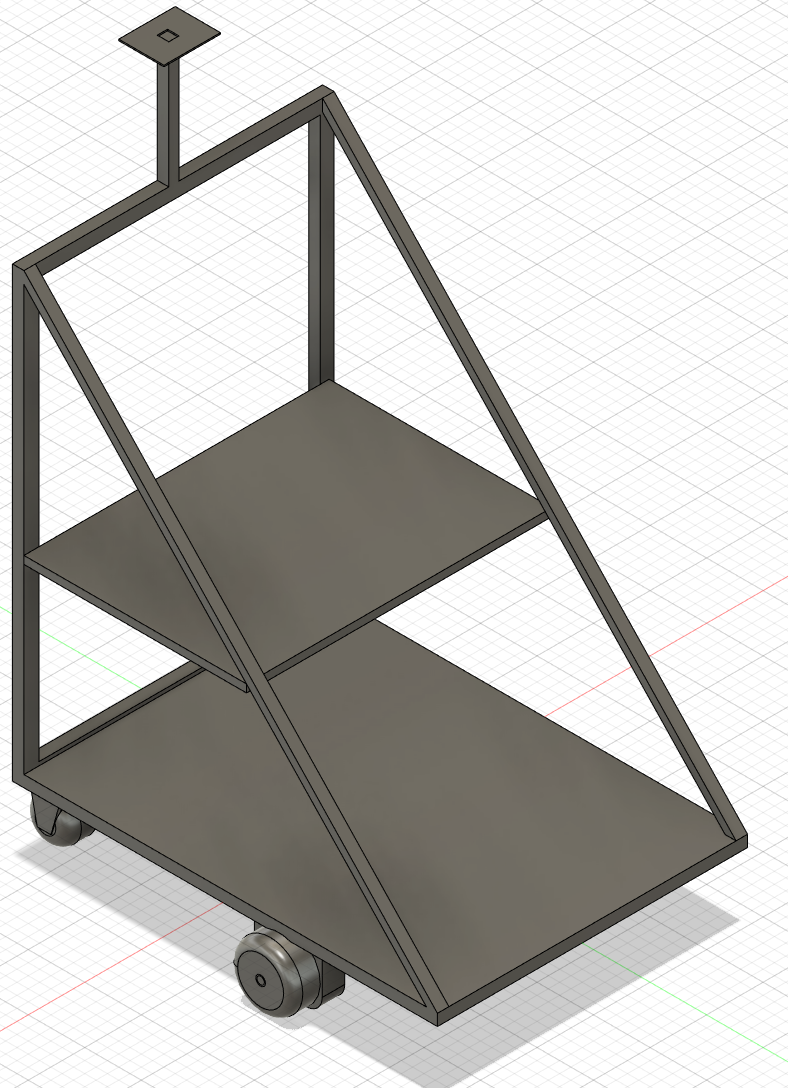
\includegraphics[scale=0.04]{images/frame/frame2.PNG}
% &
% 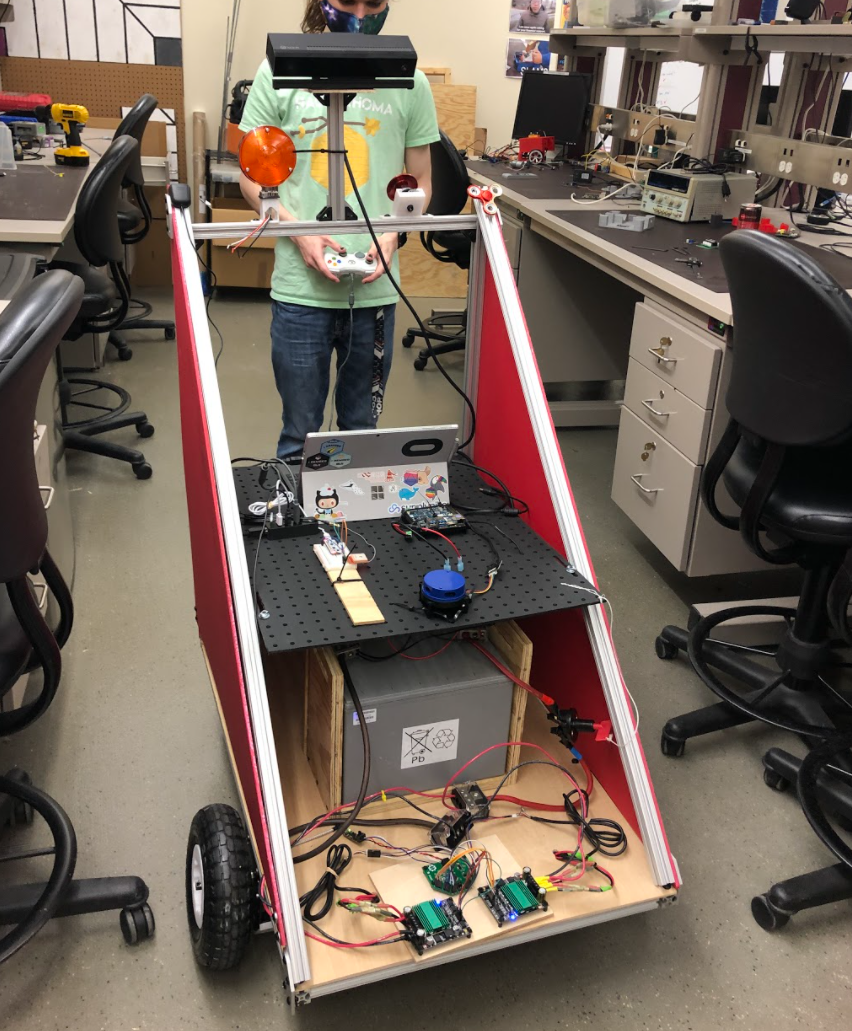
\includegraphics[scale=0.04]{images/frame/real.JPG}
% \end{tabular}
% \caption{The basic structure of the robot.}
% \end{figure}

\begin{figure}[h]
  \centering
  \begin{minipage}[b]{0.35\textwidth}
    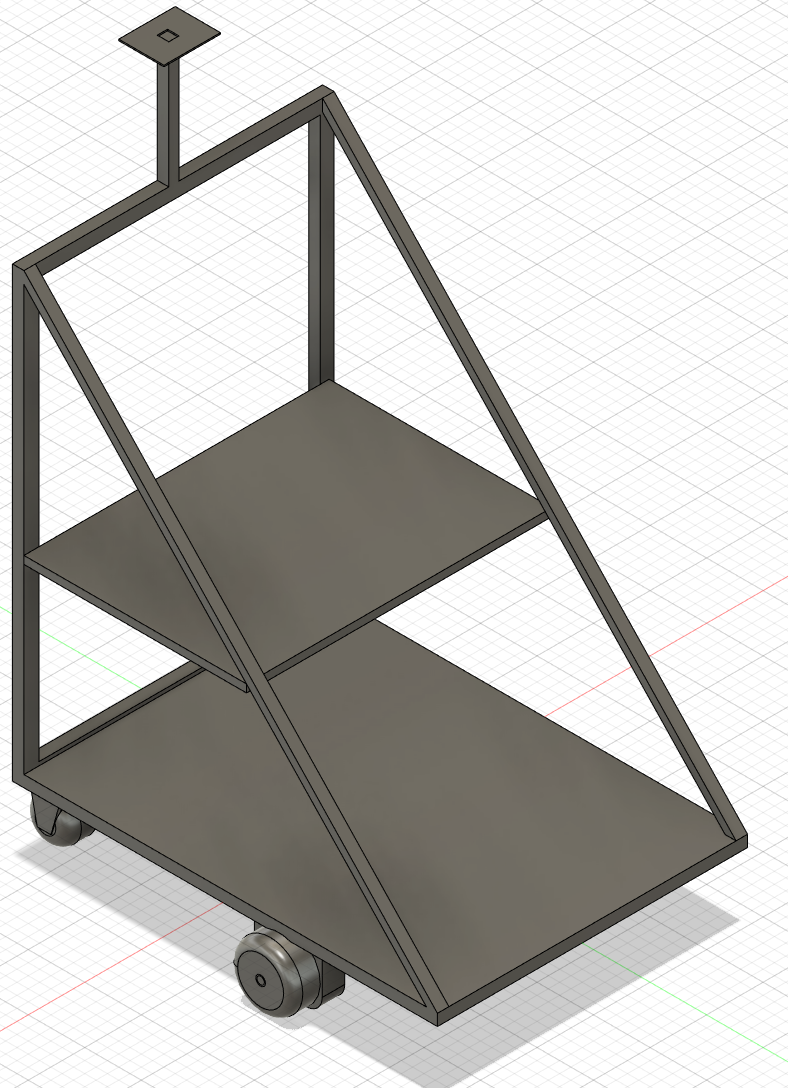
\includegraphics[width=\textwidth]{images/frame/frame2.PNG}
    \caption{CAD model for the basic structure.}
  \end{minipage}
  \hfill
  \begin{minipage}[b]{0.4\textwidth}
    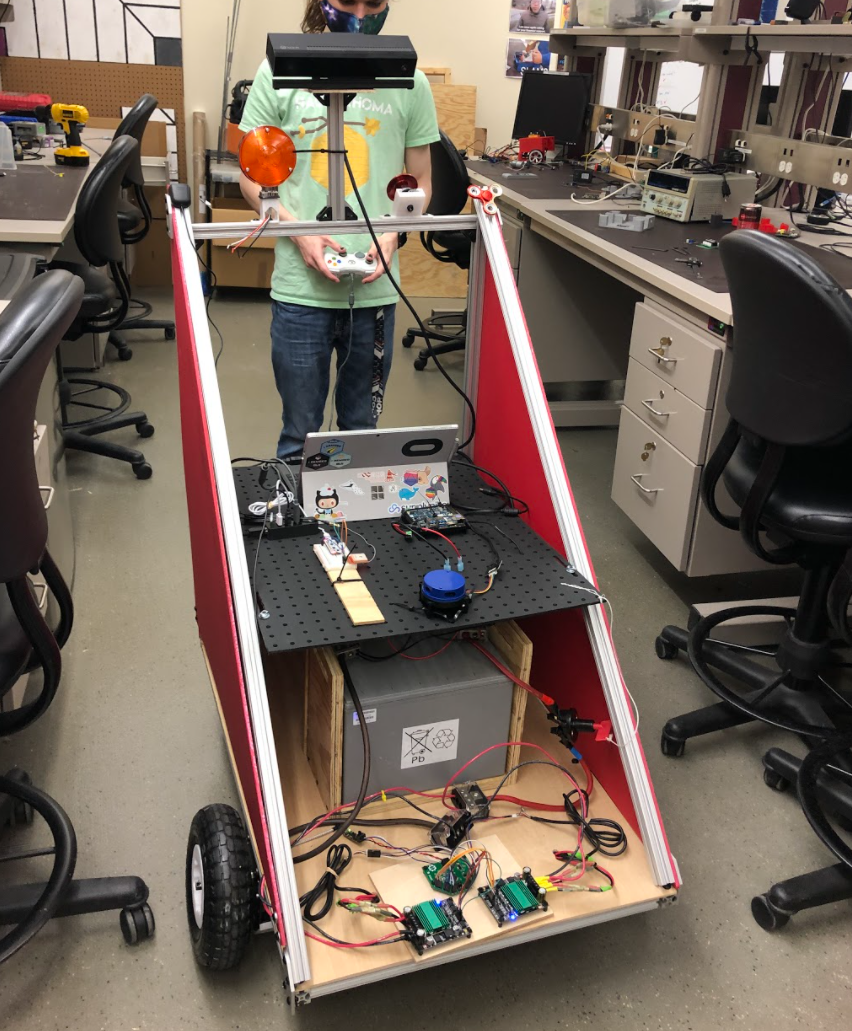
\includegraphics[width=\textwidth]{images/frame/real.PNG}
    \caption{Physical robot with most components installed.}
  \end{minipage}
\end{figure}

% \begin{figure}[h]
%     \centering
%     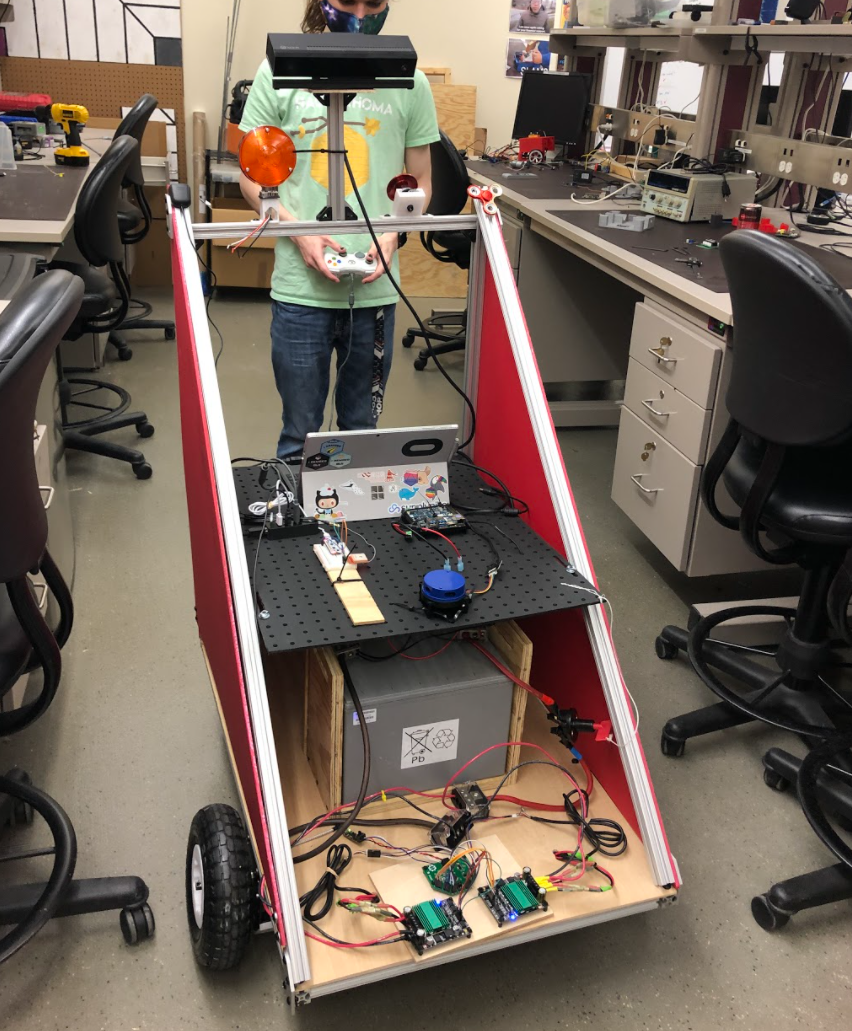
\includegraphics[width=0.4\textwidth]{images/frame/real.PNG}
%     \caption{Basic aluminum frame of the robot, with a wooden base panel, polyboard shelf for the electronics, and red acrylic paneling on the sides.}
% \end{figure}

The basic frame of the robot is composed of aluminum T-slot channels in two triangles connected at the three vertices, with additional support trusses on the underside. The base of the robot is a wooden panel supported underneath by several aluminum channels. On these channels are mounted two casters at the back corners and the two gearboxes about 2/3 of the way up the robot. We decided on this position as a good balance between perfect zero-point turns (wheels at midpoint) and the most usable space on the robot for heavy payloads (wheels at the front). We position our heavy robot battery on the wooden base directly over the drive axle and load the cinder block behind it, between the two ``axles''.

We've mounted a polyboard shelf 15" above the wooden base, which we use to attach most electronics. This height was chosen to give a few inches of clearance above our battery box. The holes in the polyboard are helpful for wire and cable routing, and there are more significant gaps at the sides for connectors too big for the holes. This shelf sticks out 5" beyond the aluminum slant to mount the LiDAR above the drive axle with as little obstruction as possible. This gives us near 180 degrees LiDAR data. The LiDAR mount is shown in FIG. \ref{fig:mount:lidar}.

\begin{figure}[h]
    \centering
    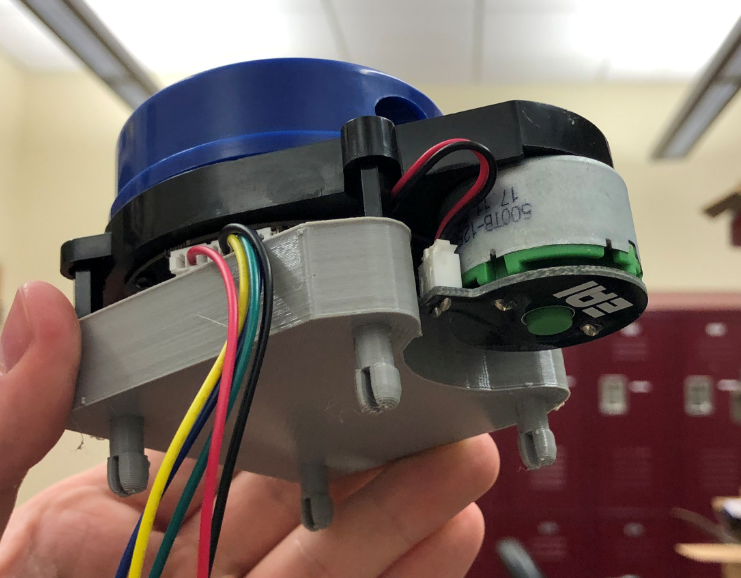
\includegraphics[width=0.4\textwidth]{images/lidar_mount.PNG}
    \caption{3D printed LiDAR mount easily attaches to the polyboard shelf.}
    \label{fig:mount:lidar}
\end{figure}

The camera we're using is the X-Box Kinect 2, which is mounted at the top of the tall pole at the rear of our robot to give it the best view. We mount it onto a small flat piece of wood to improve stability.

We have no formal suspension, opting for flexible mounting of components and built-in tolerance in code for shaky camera and LiDAR data.

The weatherproofing plan consists of enclosing the chassis by acrylic panels on all sides, with caulk or foam filling the gaps. Our concerns with fully enclosing the robot include accessibility to components for maintenance and heating inside the chassis. We subvert this first issue by including hinged panels on areas that will need access, and designing the layout of the components within the robot to be centralized to these such areas. All electronics are located on the shelf midway up the robot with the exception of the motor controllers, which are at the very front of the robot. This means we could ensure everything is accessible from the slanted front face when it is open.

\begin{figure}[h]
    \centering
    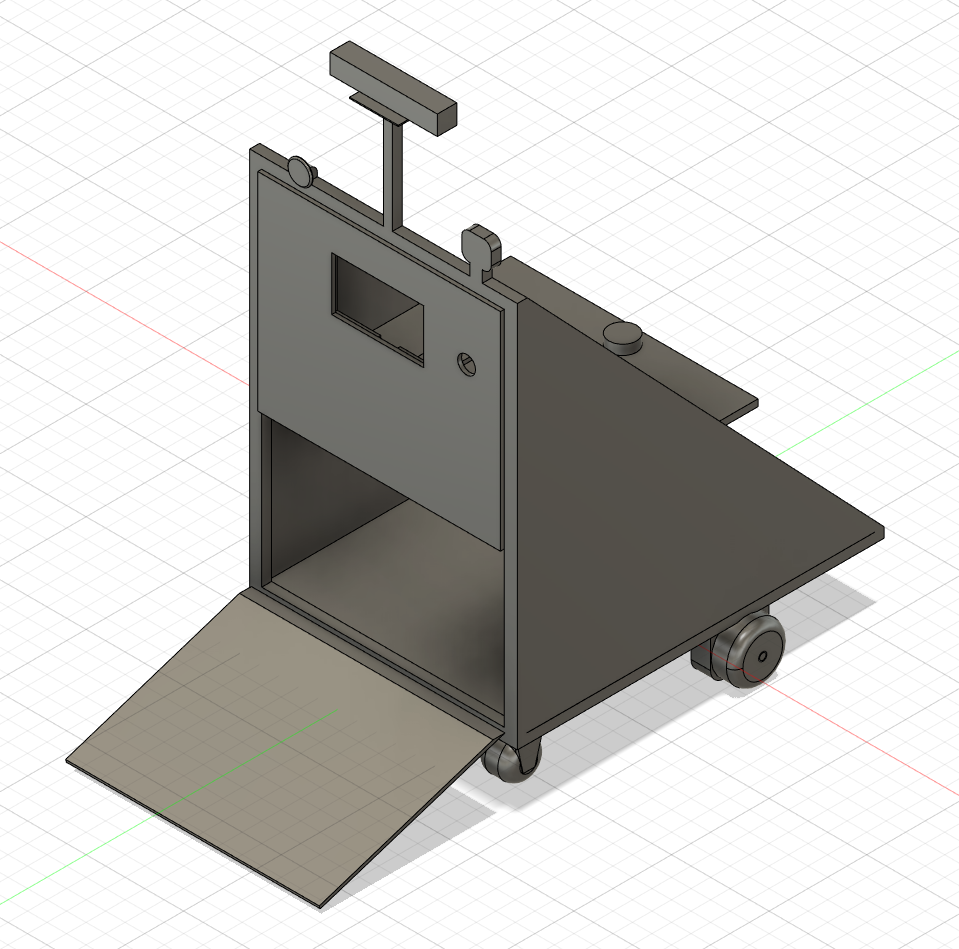
\includegraphics[width=0.5\textwidth]{images/frame/frame5.PNG}
    \caption{The lower-back panel hinges open to provide a loading point for the robot battery and the cinder block payload. The rectangular gap on the upper part is for a screen that shows debug information while the robot runs.}
\end{figure}

To help with air circulation inside the robot, we leave some small downward-facing gaps near the upper part of the robot, which lets air passively circulate with minimal danger of rainfall entering. We do not believe active cooling (i.e., with fans) is necessary for our setup. Since we need to partially disassemble the robot for our travel to and from the competition, we will bring the caulk and, only if necessary, apply it to gaps between paneling on the lower part of the robot, and seal wire-access holes on the base with caulk or hot glue. We aren't worried about water entry through the lower-rear hinged panel since it will be adjacent to the cinder block and not very close to any electronics. 

The main concern for waterproofing with our sleek design is the LiDAR. It needs to be accessible to the open air and cannot be surrounded by plexiglass, plastic, or even saran wrap. We have designed a covering to be installed directly over it to be used for light rain, but if the weather worsens, we will be removing the LiDAR for its safety. As will be discussed in later sections, our robot can function even if individual modules are removed. Our software is robust with multiple different input sources, so it will still perform without LiDAR data.
%\clearpage
\section{Electrical Design}
\subsection{Overview}
The 2021 year is our first year competing, so the electrical design of the robot focused on safety and reliability. The robot's electrical system is comprised of several modules that perform various tasks using custom PCBs with dedicated STM32 microcontrollers. The modules use the CAN bus to communicate with each other, and are made to be easily replaceable in case of failure. The robot can still function successfully if a module is disconnected. It also has several different safety features that increase reliability through redundancy.

\subsection{Power distribution}
The robot is powered using a single 12V 82Ah lead-acid battery. The type of battery we chose is used for electric power forklifts in the industry. The battery is designed to have a life of at least ten years. The voltage is stepped down or boosted as needed. Our nominal current consumption is calculated to be around 22 Amps when the robot moves at a rate of 5 MPH. The robot can operate continuously for 220 minutes using the 80Ah battery at the nominal current consumption rate. The battery has a recharge time of 24 hours. The robot was initially designed for the batteries to be hot-swapped, but the battery capacity has made that feature unnecessary. The power is distributed through Molex cables connected to every module with fuses for safety.
\subsection{Electronics Suite}

\subsubsection{Overview}
The robot has several modules and sensors throughout the system. The CAN bus allows devices to work independently, so if one device malfunctions, then the rest of the robot is functional.

\subsubsection{CAN molex}
We are using Molex connectors and cables to distribute power throughout the board. Each CAN Molex cable has six wires: 12V power, 5V power, ground, 3.3V E-stop signal, CAN high, and CAN low. The CAN Molex cable is an easy-to-route solution that provides a safe and reliable method to distribute power and data through the robot.

\subsubsection{Motor Control}
We use an STM32f103 microcontroller for our motor control. The calculated speed of each wheel is sent over the CAN bus, and the motor control board sets the speed of each wheel, respectively. Each set of wheels has an encoder that we use as feedback to control and correct the rate using a software PID controller on the STM32 chip.

\begin{figure}[h]
\centering
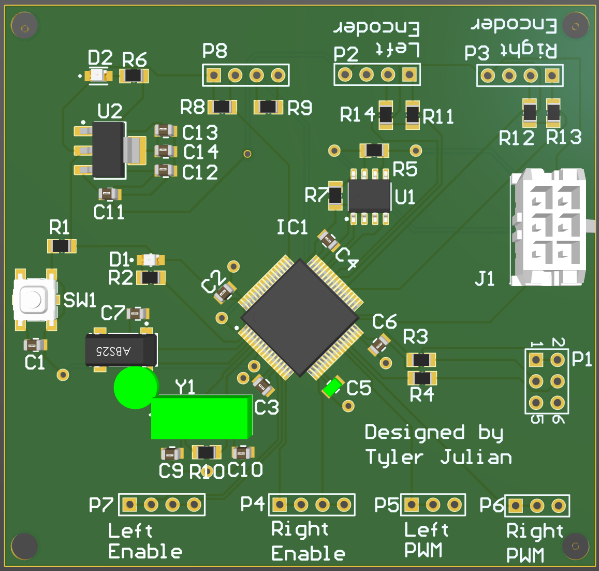
\includegraphics[width=0.3\textwidth]{images/electrical/motorControl.PNG}
\caption{The motor control PCB with the CAN Molex and STM32f103 chip.}
\end{figure}

\subsubsection{GPS}
The PCB we designed for the GPS module is based upon an STM32 microcontroller architecture. The microcontroller receives serial data from the sensor and then transmits it via CAN to our onboard computer for processing.

\begin{figure}[h]
\centering
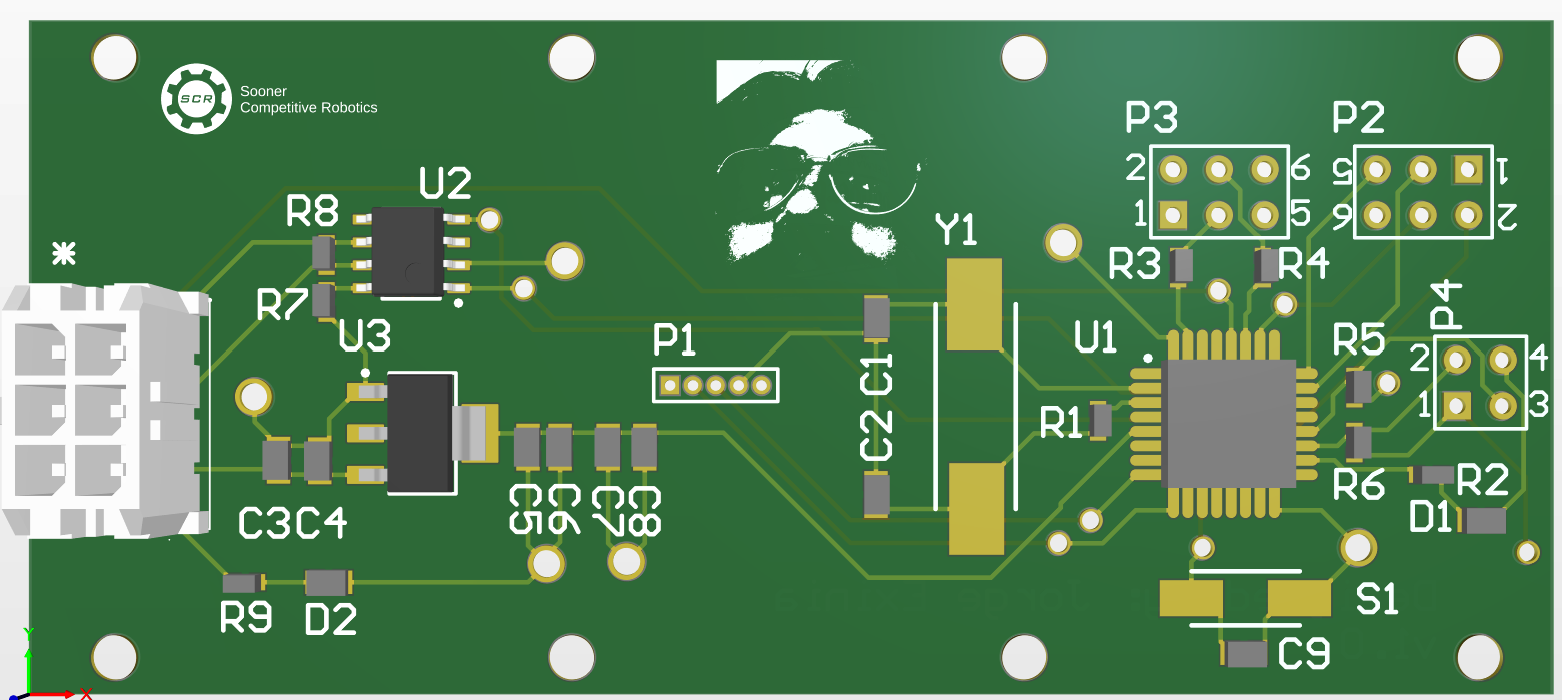
\includegraphics[width=0.3\textwidth]{images/electrical/gps.png}
\caption{The GPS PCB.}
\end{figure}

\subsubsection{Safety lights}
The PCB for the safety lights module is also based on an STM32 microcontroller architecture. An external 12V light is connected to the printed circuit board that is then switched on and off depending on the navigation state of the robot. This is done using a microcontroller and a MOSFET.

\begin{figure}[h]
\centering
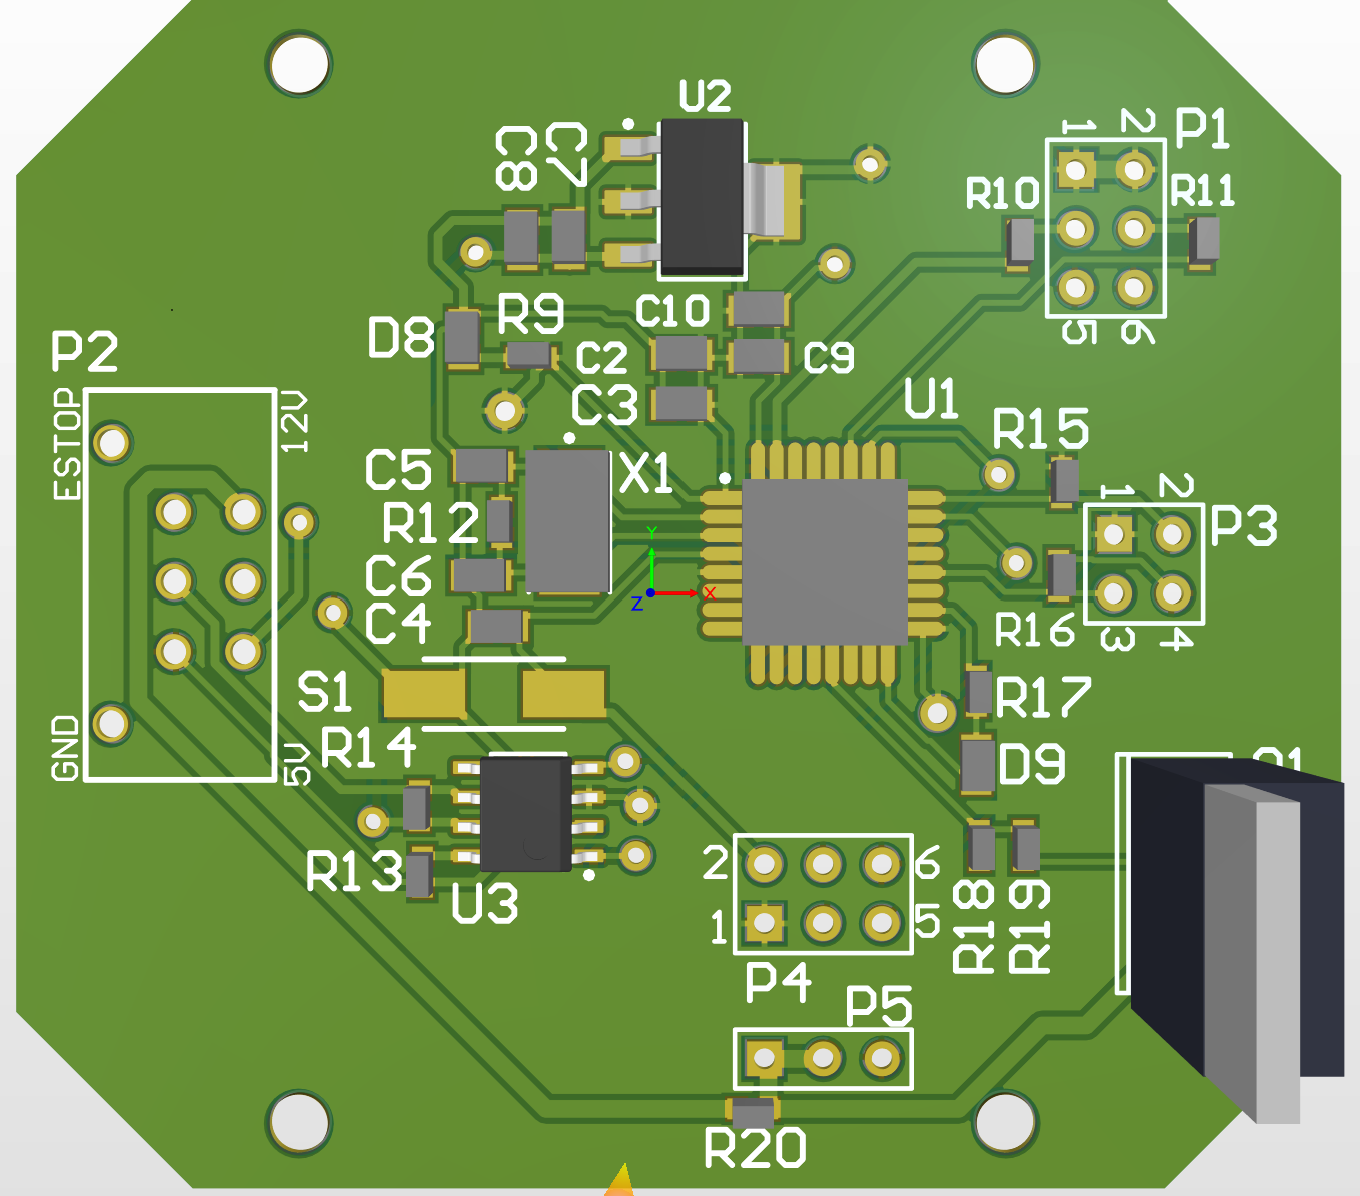
\includegraphics[width=0.3\textwidth]{images/electrical/SafetyLightsPCB.png}
\caption{The safety lights PCB.}
\end{figure}

\subsubsection{Remote E-stop}

Our remote E-stop system consists of two PCBs that communicate over radio to relay information about the E-stop and more. Each PCB uses an Adafruit Feather M0 LoRa as its microcontroller with a built-in radio transceiver for communication between the two. One PCB lies on the robot and waits for the E-stop radio signal. Once it receives the signal, the robot-wide E-stop signal is set, and the robot stops. The other PCB lies in a 3D printed remote control that will send the radio E-stop signal. The signal is sent with the press of the main button. Additionally, the remote also shows information about whether the robot is connected to the remote and acts as the start button to launch the robot into autonomous mode.

Both parts of the remote E-stop are constantly communicating, and if this connection is broken and a signal from the remote is not received after 2 seconds, E-stop will be initiated on the robot.

\begin{figure}[h]
\centering
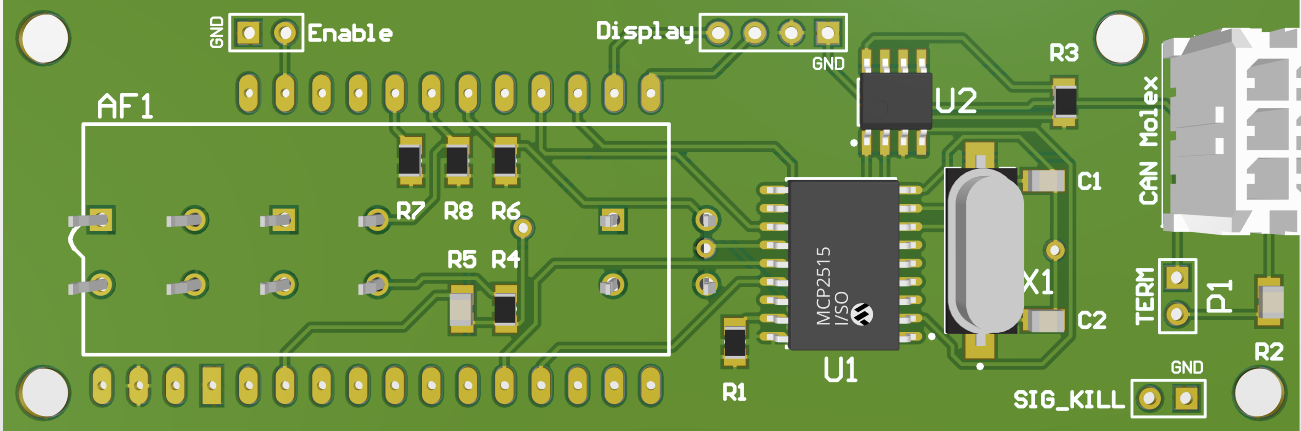
\includegraphics[width=0.3\textwidth]{images/electrical/estop.PNG}
\caption{The remote E-stop PCB.}
\end{figure}

\subsubsection{Hardware E-stop}
We convert the 3.3V E-stop signal to 24V to control an automotive contactor initially made for Toyota vehicles that cuts power to the motors when the E-stop signal is low or disconnected.

\subsubsection{IMU}
The Inertial Measurement Unit (IMU) is connected to the ODROID using USB. The ODROID processes the IMU data for use in our localization.

\subsubsection{LiDAR}
The LiDAR is connected to the ODROID using USB. The ODROID processes the LiDAR data and uses it for obstacle avoidance.

\subsubsection{Kinect}
We are using the X-Box Kinect 2 as a USB camera for our lane detection and other computer vision needs.

\subsection{Safety Devices}
\subsubsection{Emergency stops}
The robot has three ways to stop the robot:
\begin{itemize}
    \item a remote E-stop button
    \item a hardware E-stop button
    \item a key that cuts power to the entire robot when removed
\end{itemize}

The remote E-stop board generates a 3.3V E-stop signal that is sent through the entire robot. The robot is operational when the E-stop signal is high, but is not functional when the signal is low. The robot will shut down if it hasn't received a heartbeat message from the remote E-stop. The robot actively avoid obstacles using the LiDAR as well.

The robot has several systems that causes it to shut down for safety reasons. The first and most significant is the industrial contactor that cuts power to the motor controllers and motors when the E-stop signal is low. The second motor shutdown feature is a software stop that sets the motors speed to zero when the E-stop signal is low. The third feature isn't reliant on the E-stop signal. Emergency and mobility stop messages are sent through the CAN bus that disables the motors and sets the speed to zero. 

The three different systems make the robot safe and reliable with multiple layers of redundancy. 


\subsubsection{Safety Lights}
Our lights comply with the rules of competition. The lights remain solid when the robot is on and in manual mode, and strobe when the robot is autonomous. We use a 12V external light that is designed for semi-trucks and nighttime driving. With this in mind, there are not any visibility concerns.  The light is controlled with an STM32 microcontroller and a MOSFET. The MOSFET is rated for up to 50 Amps, which exceeds the current draw of the light.  


%\clearpage
\section{Software Design}

\subsection{Overview}

Our robot's software uses Robot Operating System (ROS), a popular robotics middleware, as its core. There are several \textit{nodes} which each handle a distinct task and can publish data for other nodes and subscribe to data that has been published. These nodes roughly outline all the different components of our overall software base, and individual areas are detailed in the following subsections. The information flow is shown in FIG. \ref{fig:block:software}. Our entire codebase is open-source and is available at \url{https://github.com/SoonerRobotics/igvc_software_2021}.

\begin{figure}[h]
    \centering
    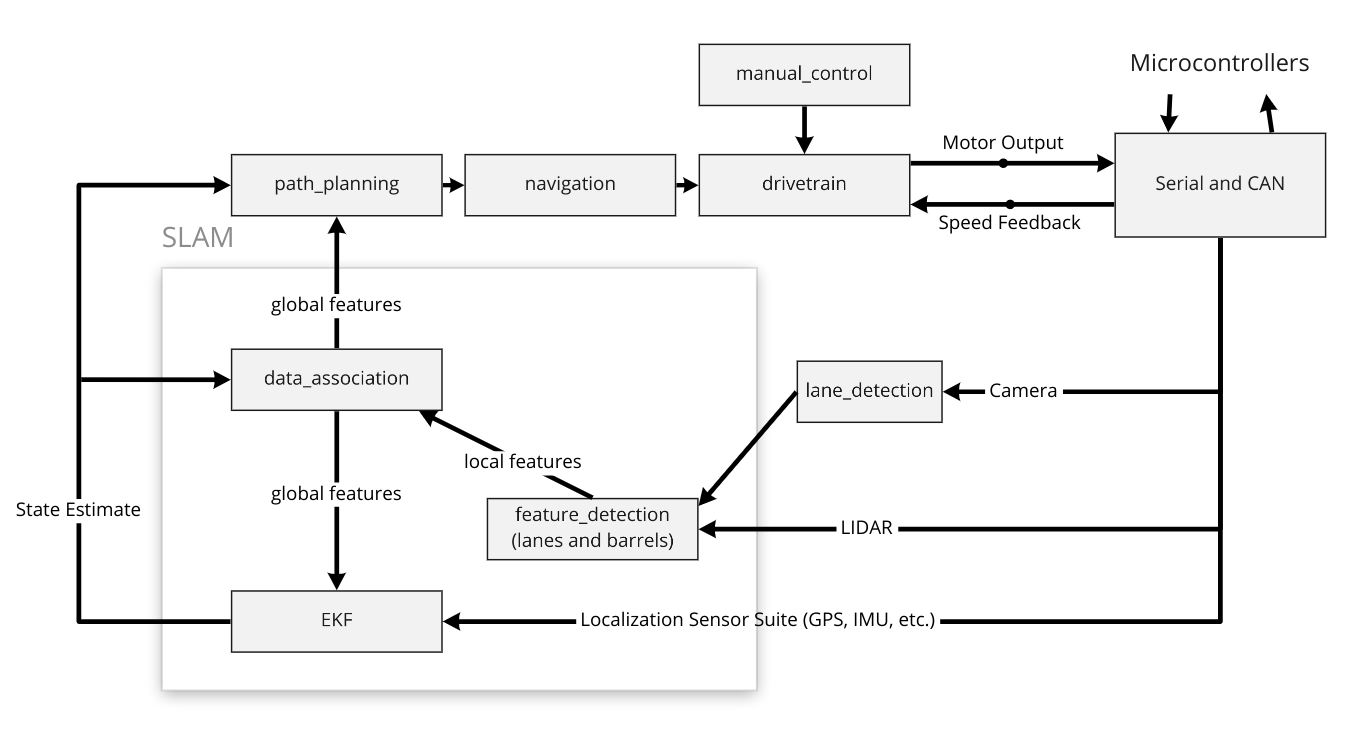
\includegraphics[width=0.9\textwidth]{images/software/software_block.png}
    \caption{Our software block diagram.}
    \label{fig:block:software}
\end{figure}

\subsection{Lane Detection}

To accomplish the difficult task of detecting the lanes, we experimented with two methods. The first method involved using standard computer vision techniques, and the second method was a convolutional neural network (CNN). Both ways perform the same overall function of taking an RGB image from the robot's Kinect camera and creating a black and white image with white identifying the lanes. 

Additionally, we perform a simple perspective correction to transform the image to a bird's eye view perspective. This allows us to directly use the image in the path planning step as described later.

\subsubsection{Computer Vision Techniques}

Our computer vision method used a variety of techniques chained together to produce our lane-segmented image. This consisted of applying thresholds to the HSV values to target pixels that match those of the lanes. This method was alright, but it was hard to find the balance between complexity in design and oversimplification of the results.

\subsubsection{Convolutional Neural Network}

Our second attempt used a convolutional neural network to detect lanes. The architecture we chose is a standard U-Net architecture which performs image segmentation well \cite{UNet}. We implemented the architecture in TensorFlow as it is easy to create models in and adjust to our needs quickly. We collected video of chalked grass using our robot's camera and then labeled the lane pixels in each image by hand to train the model. We then trained the model on these images, and we were able to produce the following results.

\begin{figure}[h]
    \centering
    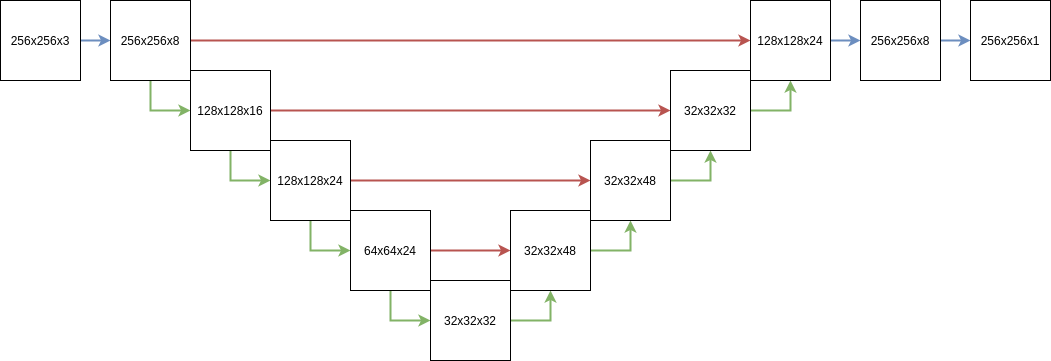
\includegraphics[width=0.7\textwidth]{images/software/unet.png}
    \caption{Our U-Net architecture which takes RGB images and outputs a black and white image of where the lanes are.}
\end{figure}

To ensure the CNN did not develop a simple thresholding algorithm, we took several different datasets in different weather conditions, with differently colored obstacles, and with people in the frame. The CNN succeeding with this amalgam of training data gives us high confidence that it will successfully identify all lanes and only lanes for most reasonable weather and brightness conditions.

\begin{figure}[H]
    \centering
    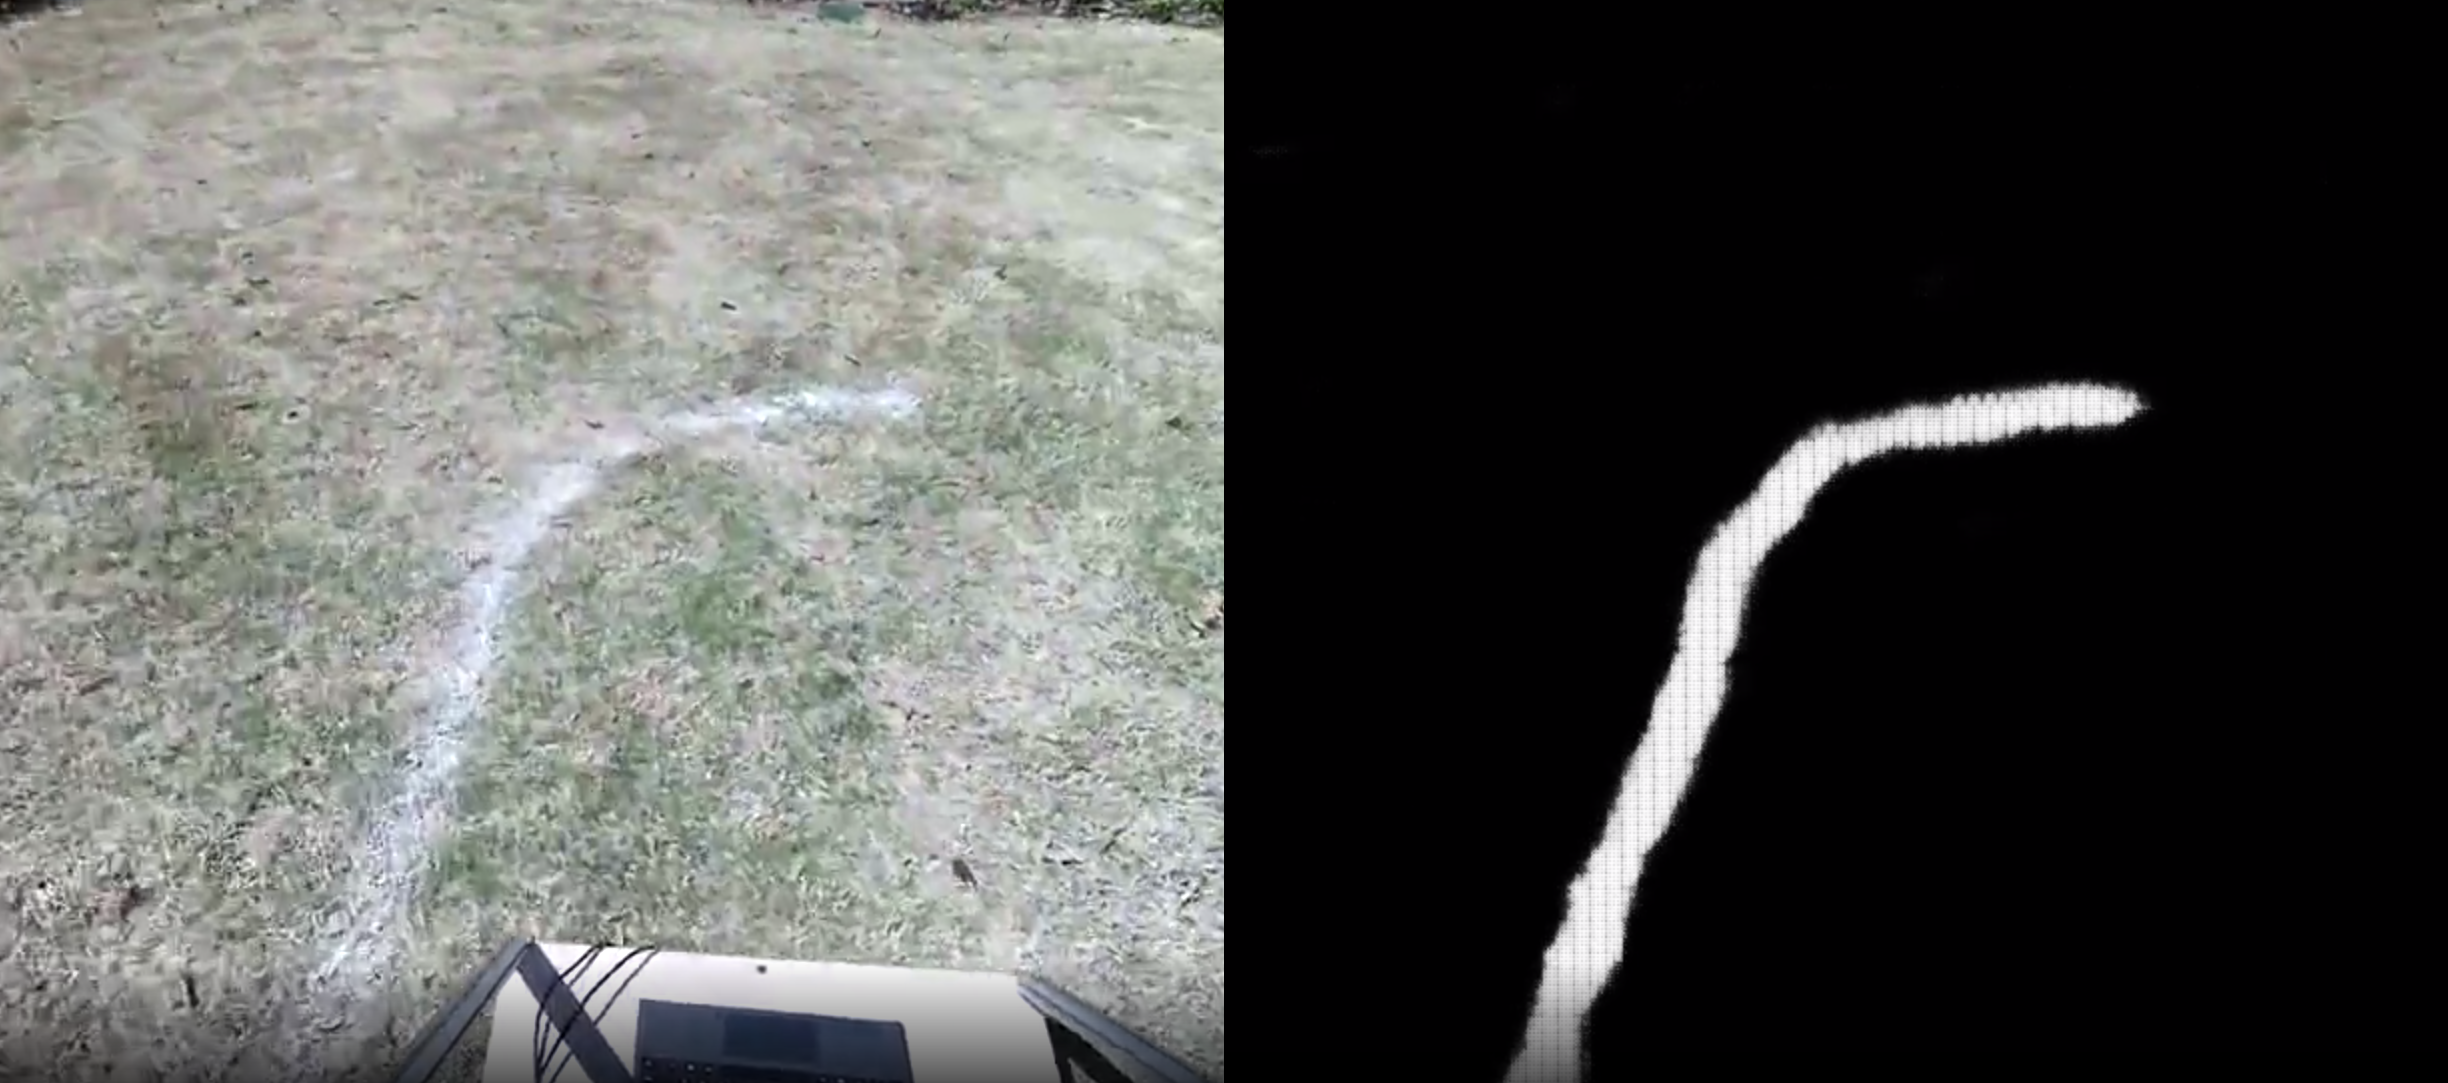
\includegraphics[width=0.5\textwidth]{images/software/unetexample.png}
    \caption{Cropped example showing the output of our U-Net on an image.}
\end{figure}

\subsection{Localization}

We use an Extended Kalman Filter (EKF) to track and update our \textit{state} estimation at every timestep. A Kalman Filter is a sensor fusion algorithm that performs a weighted average over time to balance measurements and predictions to track some state variables accurately. Our state, $\boldsymbol{X}$, consists of all variables we want to keep track of, plus all variables necessary to update the former. The state is a column vector,

\begin{equation}
    \boldsymbol{X} = \begin{pmatrix}
    x & \dot{x} & y & \dot{y} & \phi & \dot{\phi} & v_l & v_r
    \end{pmatrix} ^T
    \textrm{ ,}
    \label{eqn:kf:X}
\end{equation}
where $x$ and $y$ are the component positions in meters, $\dot{x}$ and $\dot{y}$ are the component velocities in meters per second, $\phi$ is the global heading (yaw) in degrees, $\dot{\phi}$ is the yaw rate, and $v_l$ and $v_r$ are the angular velocities of each wheel. 

To create and update this state, we receive input from several different sensors on our robot. We have available GPS, IMU, LiDAR, camera, and encoder data and choose only to use a subset of these. The reason is that for our use case, the EKF will only really come into play once we reach No Man's Land, so it isn't our highest priority. The measurement vector that we track each timestep is represented in Equation
(\ref{eqn:kf:Z}). It is possible to obtain and update our state with as little data as the wheel angular velocities and the yaw.

\begin{equation}
    \boldsymbol{Z} = \begin{pmatrix}
    v_l & v_r & \phi
    \end{pmatrix} ^T
    \label{eqn:kf:Z}
\end{equation}

We convert measurements to equivalent state values via Equation (\ref{eqn:kf:dynamics}). Note that we use a constant velocity model; this means the EKF assumes the velocity is constant, and any deviation from this is noise. The measurements will prod the correct evolution in these values, so this simplification works just fine.

\begin{equation}
    v = \frac{1}{2} \cdot \textrm{WHEEL\_RADIUS} \cdot (v_l + v_r)
    \label{eqn:kf:dynamics}
\end{equation}

\begin{equation*}
    \begin{cases}
    x = x + \dot{x} \Delta t\\
    \dot{x} = v \cos{\phi}\\
    y = y + \dot{y} \Delta t\\
    \dot{y} = v \sin{\phi}\\
    \phi = \phi - \dot{\phi} \Delta t\\
    \dot{\phi} = \frac{\textrm{WHEEL\_RADIUS}}{\textrm{WHEELBASE\_LEN}} \cdot (v_l - v_r)\\
    v_l = v_l\\
    v_r = v_r
    \end{cases}
\end{equation*}

The true benefit of the EKF comes when we dynamically increase the size of the state during landmark detection (from the LiDAR data). We add the $x$ and $y$ coordinates of the center of each landmark to the state and track this throughout the rest of the EKF runs. When we identify an obstacle, we can either add new values to the state or update existing values if we determine this landmark has been seen before. Landmarks, in this case, are primarily the traffic barrels that clutter the course and No Man's Land. 

When a new obstacle is added, we can assume it has no covariance with any other variables already in the state. This makes dynamicism very simple, as our Jacobian matrix will look the same, plus two additional rows and columns; all new entries other than the 2x2 in the lower right corner will be zero, and all existing entries are unaffected. 

The Jacobian is used when updating the state at each timestep and calculating the \textit{Innovation}, the difference between our predicted state and the new measurements. We create the initial Jacobian for our state using the Python package SymPy that is very good at symbolic calculations. We can make some assumptions about the covariance of each $i$th landmark's $x_i$ and $y_i$ positions, informed by our values for the robot's $x$ and $y$ in our original state. This is very helpful for computation time because we can manually create a new Jacobian when necessary rather than recreating it from scratch using SymPy and converting the symbolic representation to equations in our C++ node.

\subsection{Path Planning and Navigation}

Our goal is to navigate the course by sending control signals determined by the data from our sensors. Because it is our first year at this competition and we have much to learn, we decided to focus on building a robust and straightforward path planning and navigation system rather than using more complex algorithms. We hope to enhance this portion of our software design significantly in future years.

\subsubsection{Path Planning}

Our robot begins its decision-making process by taking in all the filtered sensor data. We take the laserscan data from the LiDAR and the detected lanes from our CNN, and combine them into a 2D occupancy grid detailing where the robot should not move. We then further transform this grid by marking each cell within a specified distance of an obstacle as occupied. This gives us a configuration space grid that lets us treat our robot as a single point to use standard path planning algorithms on this map without worrying about our robot getting too close to an obstacle. Finally, we run D* Lite on the final grid to give us a path from where the robot currently is to an ``ideal'' position \cite{DStar}. The ideal location is chosen by spotting a specified distance forward that is not inside an occupied grid space. As a result, our robot can only progress through the course and does not retain a memory of the overall course or where it has been, another feature we plan on improving significantly next year.

As a simplification to the EKF, we reset its state every time a new path is being planned, so that all positions and landmarks are tracked only for these small subpaths. This increases the accuracy at the cost of relying a bit more on the reactive behavior of the robot.

\subsubsection{Navigation}

Now that we have the path to follow, we have to create instructions for the robot to follow. To solve this, we used a simple path tracking algorithm called Pure Pursuit \cite{Pure Pursuit}. The algorithm takes the current position of the robot and the path we wish to pursue as an ordered list of points. The result is a heading that the robot should target that aims at a point on the path some short distance away from the robot. Using that heading, we can then generate motor instructions for our robot to turn the robot to face the heading. The robot always attempts to move forward but will reduce forward velocity while rotating to fit the heading.

\clearpage
\section{Failure Modes and Resolutions}

\subsection{Software Robustness}

Our robot is able to function even with the failure or removal of any physical sensor or shutdown of any software node. As we have mentioned throughout this document, we use ROS for our software architecture. If something like the main control node is somehow shutdown, the robot will continue to take in data and attempt to act on it, but the commands will not make it to the motors to induce motion. Aside from the control node, any other part of the software can randomly cease and resume functionality without completely stopping the robot. In the worst case, if only the control node is operable, we will still be able to reactively move through the course with no plan of where we are going; luckily the lanes sort of force forward progress, at least for some amount of time. If the robot reaches No Man's Land and we notice it is not pursuing a reasonable path and seems to be moving randomly, we can easily E-stop it.

The E-stop is mainly a hard stop on the basic electronic level. It is also not reversible, and the robot must be completely restarted to move again; this prevents an accidental double press from having adverse affects. Since the E-stop happens without going through the software, it will still work even if the ODROID disconnects or all the deliberative aspects of the robot somehow fail simultaneously.

% An example of our deliberative redundancy is the LiDAR. If the physical LiDAR is unplugged and removed from the robot, as we plan to do in case of heavy rain, or it becomes damaged while the robot is running, everything else will continue working. Because of the pub/sub nature of ROS, this would simply amount to one less source we receive data from; without it, the sensor fusion would be less effective, and we would be relying mainly on the camera for obstacle detection rather than both it and the LiDAR. Neither of these is desired, but they are definitely preferable to a complete fail state when any one component fails.

If our IMU or GPS sensors go out, we can gather position and velocity data from only one rather than both. If both go out, we can still proceed using dead reckoning from encoders on the drive wheels. Each missing piece of our architecture leads to worse results but preserves functionality until everything is broken, in which case we have more significant issues than robustness in the code. 

\subsection{Electronics Interconnectivity}

As mentioned in Section \ref{sec:innovations}, our electronics form an interconnected CAN network with core components at the ends. If anything nonessential breaks or becomes disconnected, even in the middle of a run, we can continue with the competition.

Our ultimate failure point would be in the case of a fault in something directly necessary for the robot's functionality; if the motor controllers break, we will not be able to drive the robot until we replace them. We have backups of such components but would not change them out until we have several minutes with our tools and the robot, likely between runs, in which to identify them as the problem and perform the swap.

\subsection{Mechanical Integrity}

We do not predict any unexpected damage to the robot that would not be immediately fixable. We have designed the robot reasonably well to have multiple points of connection and support between any given set of components. If an electronics mount breaks, we will attempt to repair it and, as a last resort, use zip ties, hot glue, or duct tape. If a panel starts to come off on a given side, we will tighten the bolts and, as a last resort, simply duct tape it to adjacent panels. Any gaps can be reduced and filled with caulk for waterproofing.

We're bringing spare tires and a bike pump, so if our wheels burst or deflate, we're prepared to remedy it. We've designed 3D printed covers for our gearboxes to keep dirt and other gunk out of them and will be printing extras to bring in case of breakage. Many different components are 3D printed, such as the onboard and remote E-Stop holders, the safety light mount, and many electronics mounts. We'll be printing and bringing extras of all these.

We will be bringing extras of all bolts, screws, nuts, washers, and other small components that could come loose and be lost. We'll also be bringing all tools necessary to install, disassemble, and repair the robot and do an inventory of everything before leaving for the competition. We're bringing extras for all the more significant components such as the motors and electronics if we're able. 


%\clearpage
\section{The SCR Simulator} \label{sec:sim}

We have a simulator made in Unity by one of our members for the explicit purpose of this team, so it satisfies everything we could want from a simulator. It integrates with ROS, so it publishes simulated sensor data via ROS topics the same way the actual sensors do. This means we can run our code with no modifications whatsoever. The control node publishes motor commands, and these commands are received by the simulator in the same way they would be on the physical robot.

This simulator also has capabilities for environment and robot customization, so we're able to update it and increase the accuracy of our testing as we finalize the size and shape of the robot, and we're able to test different light levels, lane configurations, obstacle densities, and whatever else we want.

\begin{figure}[h]
    \centering
    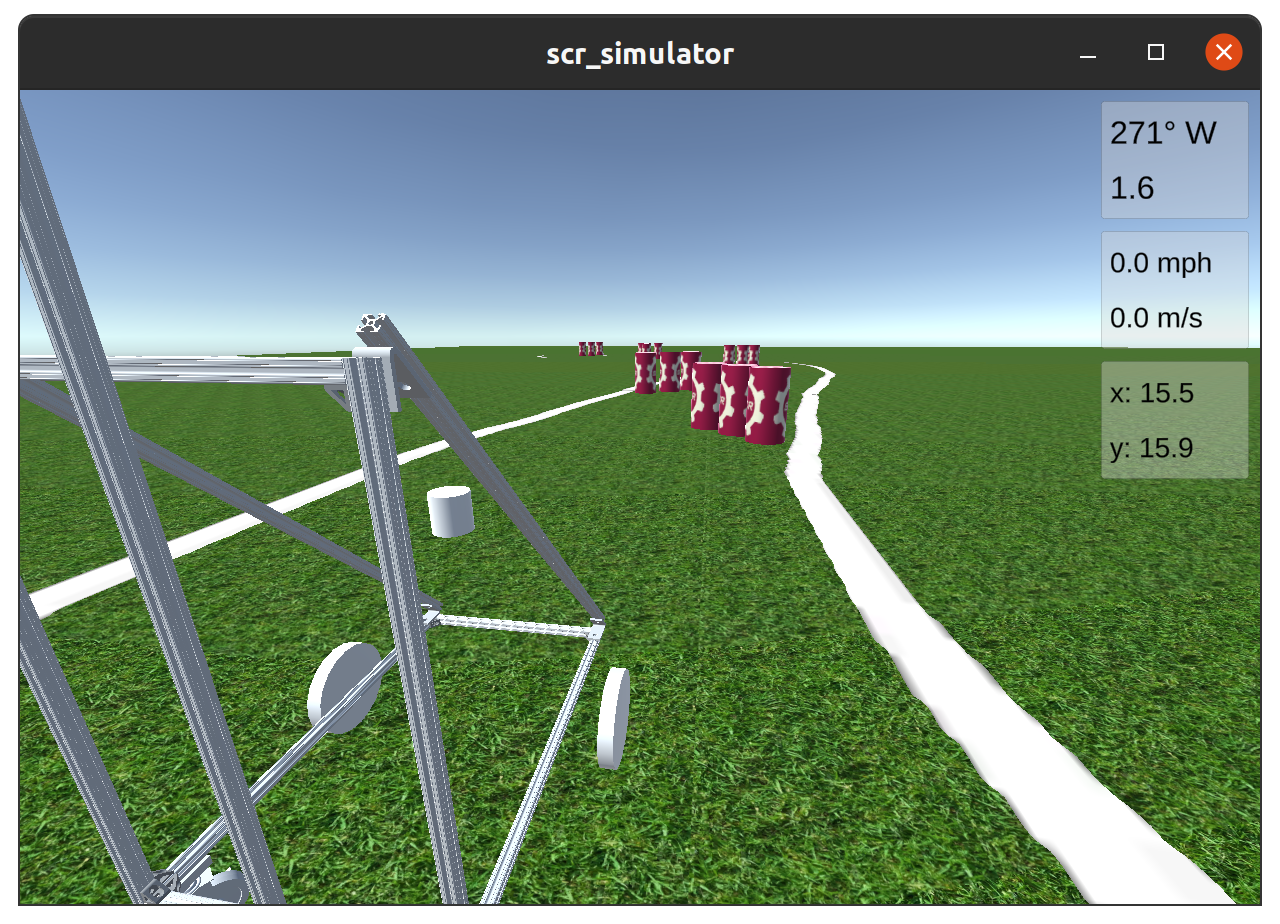
\includegraphics[width=0.6\textwidth]{images/software/sim_screenshot.png}
    \caption{Screenshot of the simulator on a map that contains both lanes and barrels.}
\end{figure}

The simulator has allowed us to make significant software progress without waiting for the robot to be built and wired, which allowed us to accomplish far more in parallel than we would have without it. We could develop our architecture and test different lane detection methods, which allowed us to settle on using a CNN and have plenty of time to flesh it out before we were setup to gather real camera footage for training data.

The simulator source code can be viewed and the latest release can be downloaded at \url{https://github.com/SoonerRobotics/scr_simulator}.
%\clearpage
\section{Performance Testing}

We have performed a lot of testing in the software realm and have had a minimally viable product in the simulator for months now. We've run the simulator in various environmental setups, from a few to many lanes, with differing gaps and with different layouts and densities of obstacles. We are pretty confident in our performance in this setting. There is noise in the simulated sensor data and controls, but we know the simulator performance is still an idealized view of our performance potential.

We frequently do drive checks in our lab and in the adjacent hallways to verify functionality as we make changes. We've done a few large-scale tests on a grassy field on which we could paint white lanes using grass chalk spray. These test days gave us insight into flawed areas that we needed to focus on with mechanical and electrical aspects. We used these days to record tons of camera data to train the CNN and simulate the competition with more realistic camera inputs than the simulator provides. 

\begin{figure}[h]
    \centering
    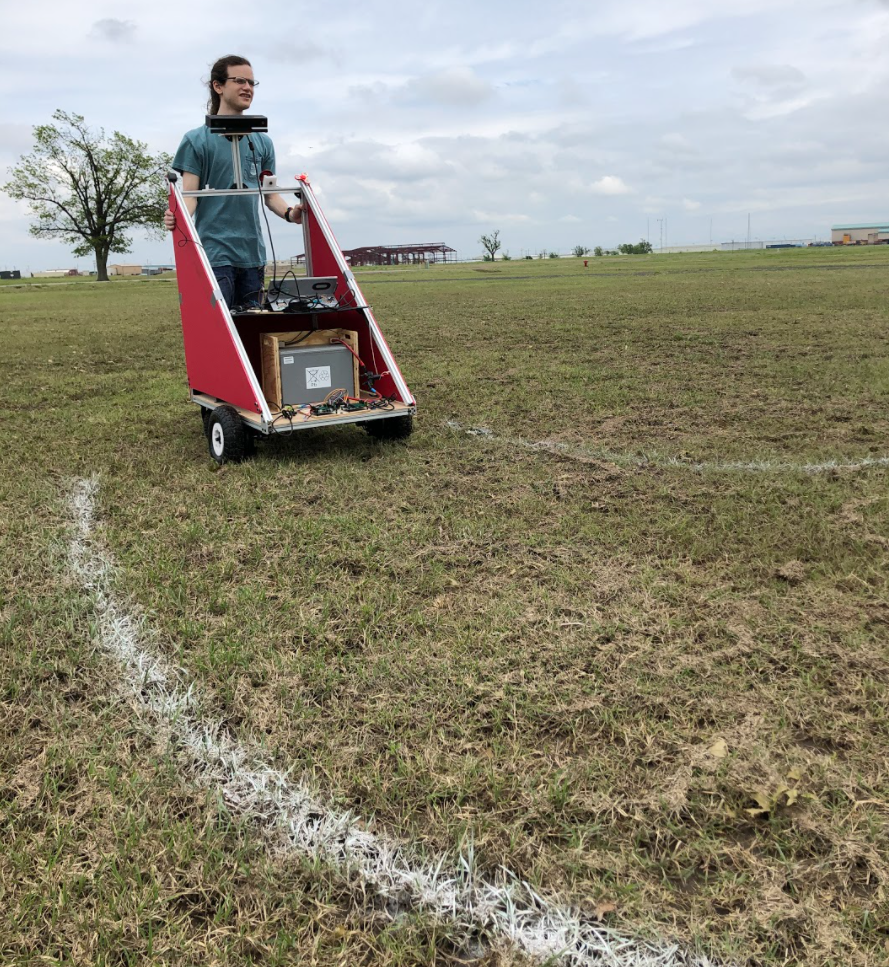
\includegraphics[width=0.4\textwidth]{images/outdoor_test.PNG}
    \caption{Outdoor test of our robot in a painted grassy field.}
\end{figure}

This testing was done before the announcement that this year's competition would take place on asphalt rather than grass, which forced us to make adjustments to both the robot design and our plans for further testing. We were still able to use the data we gathered by tinting all grass in the images to a dark grey to approximate a parking lot, but we aren't able to get free access to a real parking lot to cover lanes and paint our own. This means we can't have as much confidence in our lane detection as we could with grass, but in the worst case we will be able to take additional camera footage during the testing days once we arrive to the competition venue, and can feed that through to tune the CNN to the exact conditions we'll see in the competition.


%\clearpage

\begin{thebibliography}{7}
% Use chicago style. don't worry about order, as we can alphebatize them later if we want without messing anything up as long as \cite{} is used in text.

% example for a web reference
% \bibitem{REFERENCE_NAME}\begin{flushleft}
% Name,
% \textit{Title},
% Last modified YEAR, \url{LINK}.
% \end{flushleft}

\bibitem{UNet}\begin{flushleft}
Ronneberger, Olaf, Philipp Fischer, and Thomas Brox. \textit{U-net: Convolutional Networks for Biomedical Image Segmentation.}
International Conference on Medical Image Computing and Computer-Assisted Intervention, pp. 234-241. Springer, Cham, 2015.
\end{flushleft}

\bibitem{DStar}\begin{flushleft}
Koenig, Sven, and Maxim Likhachev. \textit{D$^*$ lite.} American Association for Artificial Intelligence, Vol. 15 (2002).
\end{flushleft}

\bibitem{Pure Pursuit}\begin{flushleft}
Coulter, R. Craig. \textit{Implementation of the pure pursuit path tracking algorithm}. Carnegie-Mellon University Robotics Institute, Pittsburgh, PA, 1992.
\end{flushleft}

% \bibitem{sympy}\begin{flushleft}
% Meurer A, Smith CP, et al.
% %Paprocki M, Čertík O, Kirpichev SB, Rocklin M, Kumar A, Ivanov S, Moore JK, Singh S, Rathnayake T, Vig S, Granger BE, Muller RP, Bonazzi F, Gupta H, Vats S, Johansson F, Pedregosa F, Curry MJ, Terrel AR, Roučka Š, Saboo A, Fernando I, Kulal S, Cimrman R, Scopatz A.
% \textit{SymPy: symbolic computing in Python.}
% PeerJ Computer Science 3:e103. 2017.
% \url{https://doi.org/10.7717/peerj-cs.103}
% \end{flushleft}

\end{thebibliography}

% make citation in text with \cite{REFERENCE_NAME}

\end{document}
